\documentclass[aspectratio=169]{beamer}
\usepackage{hyperref}
% \usepackage[T1]{fontenc}

% other packages
% \usepackage{latexsym,xcolor,multicol,booktabs}
% \usepackage{amssymb,amsfonts,amsmath,amsthm,mathptmx}
% \usepackage{calligra}
\usepackage{listings}  % graphicx, pstricks
\usefonttheme[onlymath]{serif}
% numeric tables
\usepackage{siunitx}
% algorithms
\usepackage{algorithm}
\usepackage{algorithmic}
\usepackage{amsmath}
% draw
\usepackage{tikz}
\usepackage{cases}
\usepackage{multimedia}
% \usepackage{animate}

\renewcommand{\today}{\number\year -\ifnum\month<10 0\fi\number\month -\ifnum\day<10 0\fi\number\day}
\renewcommand{\alert}[1]{\textbf{\color{stuba}#1}}
\newcommand{\ui}[2]{#1 _{\mathrm{#2}}}
% upright sub-index with variable
\newcommand{\uis}[3]{#1 _{\mathrm{#2}, #3}}

% Turn off numbering in header
\makeatletter
\let\beamer@writeslidentry@miniframeson=\beamer@writeslidentry%
\def\beamer@writeslidentry@miniframesoff{%
  \expandafter\beamer@ifempty\expandafter{\beamer@framestartpage}{}% does not happen normally
  {%else
    % removed \addtocontents commands
    \clearpage\beamer@notesactions%
  }
}
\newcommand*{\miniframeson}{\let\beamer@writeslidentry=\beamer@writeslidentry@miniframeson}
\newcommand*{\miniframesoff}{\let\beamer@writeslidentry=\beamer@writeslidentry@miniframesoff}
\makeatother

% The text inside the square brackets [] in the commands specifies their respective short versions that will appear in the header or footer of each slide in a Beamer presentation.
\author[M. Wadinger ]{Marek Wadinger, Michal Kvasnica}
% Authors with institution
% \author[M. Wadinger]{Marek Wadinger\inst{1}, Michal Kvasnica\inst{1} }
\title[Real-Time Outlier Detection]{Real-Time Outlier Detection with Dynamic Process Limits}
\subtitle{Process Control 2023}
\institute[STU]
{
\inst{} 
Institute of Information Engineering, Automation, and Mathematics \\
\textit{marek.wadinger@stuba.sk}
}
\date{}
\usepackage{STU}


% defs
\def\cmd#1{\texttt{\color[RGB]{0, 0, 139}\footnotesize $\backslash$#1}}
\def\env#1{\texttt{\color[RGB]{0, 0, 139}\footnotesize #1}}


\lstset{
    language=[LaTeX]TeX,
    basicstyle=\ttfamily\footnotesize,
    keywordstyle=\bfseries\color[RGB]{0, 0, 139},
    stringstyle=\color[RGB]{50, 50, 50},
    numbers=left,
    numberstyle=\small\color{gray},
    rulesepcolor=\color{red!20!green!20!blue!20},
    frame=shadowbox,
}

\begin{document}

\setbeamertemplate{headline}{}
\setbeamertemplate{footline}{}

\begin{frame}
    \titlepage
    \begin{figure}[htpb]
        \begin{center}
            \raisebox{-0.5\height}{
\includegraphics[width=0.1\linewidth]{figures/logos/logo_black_blue_transparent.pdf}}
            \raisebox{-0.5\height}{
\includegraphics[width=0.5\linewidth]{figures/logos/STU-FCHPT-anfh.pdf}}
        \end{center}
    \end{figure}
\end{frame}

\setbeamertemplate{headline}[smoothbars theme]
\setbeamertemplate{footline}[footline body]

% \begin{frame}
%     \tableofcontents[sectionstyle=show,subsectionstyle=show/shaded/hide,subsubsectionstyle=show/shaded/hide]
% \end{frame}


\section{Motivation}

\begin{frame}{Real World Data}
    \begin{figure}[htpb]
        \begin{center}
            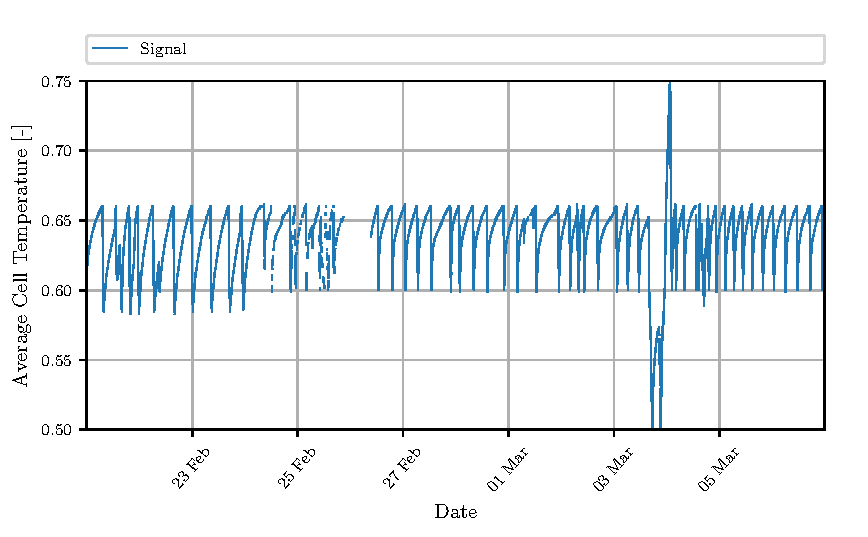
\includegraphics[width=0.75\linewidth]{../ilustrate/pc2023/bess/naive/min_signal.pdf}
        \end{center}
    \end{figure}
\end{frame}

\begin{frame}{Data with Outliers}
    \begin{figure}[htpb]
        \begin{center}
            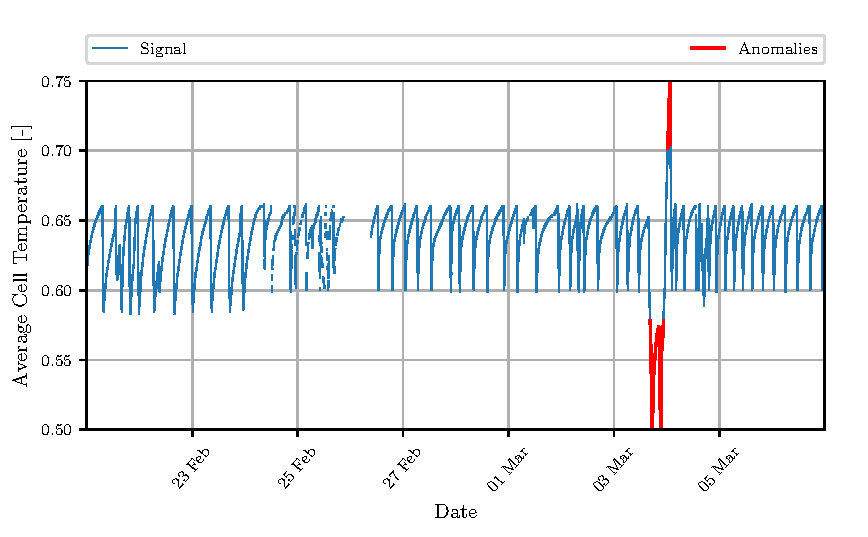
\includegraphics[width=0.75\linewidth]{../ilustrate/pc2023/bess/naive/min_anomalies.pdf}
        \end{center}
    \end{figure}
\end{frame}

\begin{frame}{Static Threshold Limits}
    \begin{figure}[htpb]
        \begin{center}
            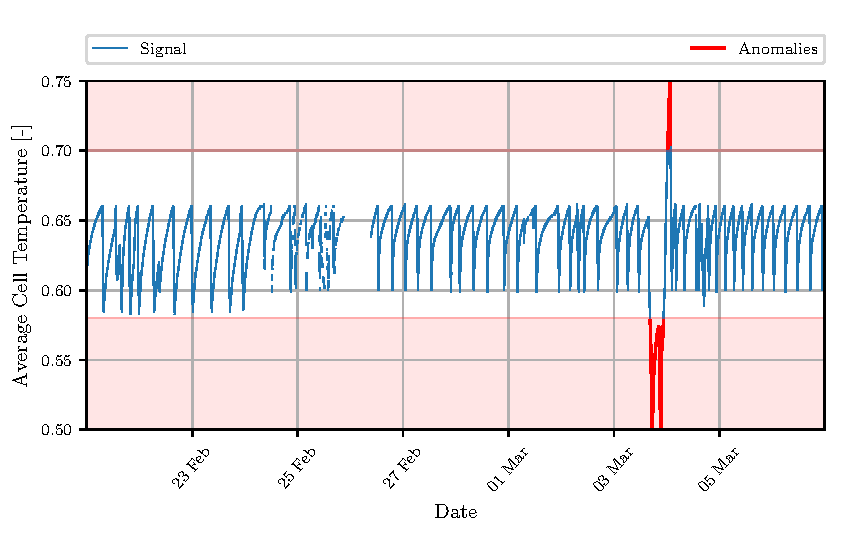
\includegraphics[width=0.75\linewidth]{../ilustrate/pc2023/bess/naive/min_thresh.pdf}
        \end{center}
    \end{figure}
\end{frame}

\begin{frame}{Static Threshold Limits}
    \begin{figure}[htpb]
        \begin{center}
            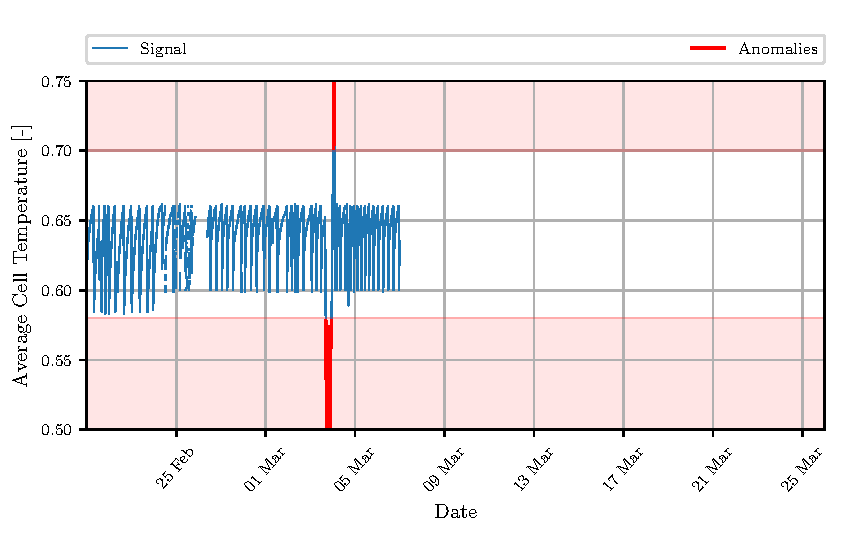
\includegraphics[width=0.75\linewidth]{../ilustrate/pc2023/bess/naive/pred_thresh.pdf}
        \end{center}
    \end{figure}
\end{frame}

\begin{frame}{Comming Problem}
    \begin{figure}[htpb]
        \begin{center}
            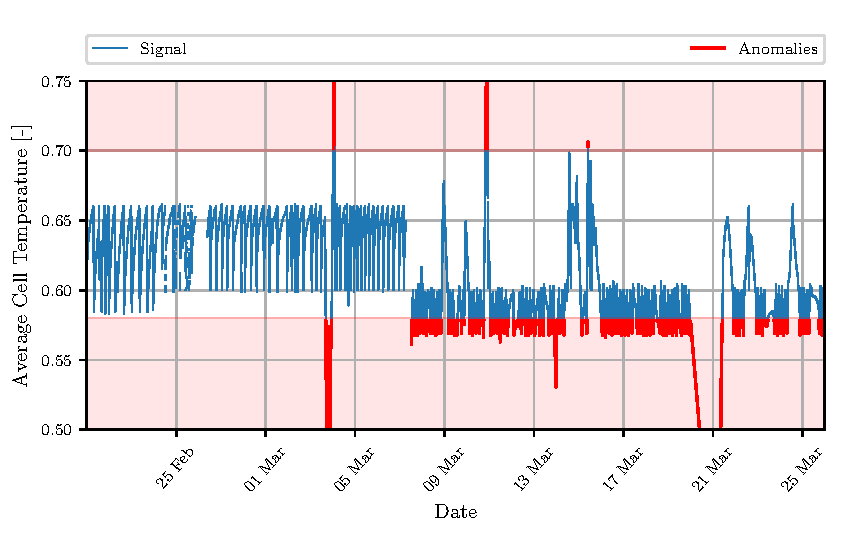
\includegraphics[width=0.75\linewidth]{../ilustrate/pc2023/bess/naive/full_thresh.pdf}
        \end{center}
    \end{figure}
\end{frame}

\begin{frame}{Control Engineering Meets Artificial Intelligence}
    \begin{figure}[htpb]
        \begin{center}
            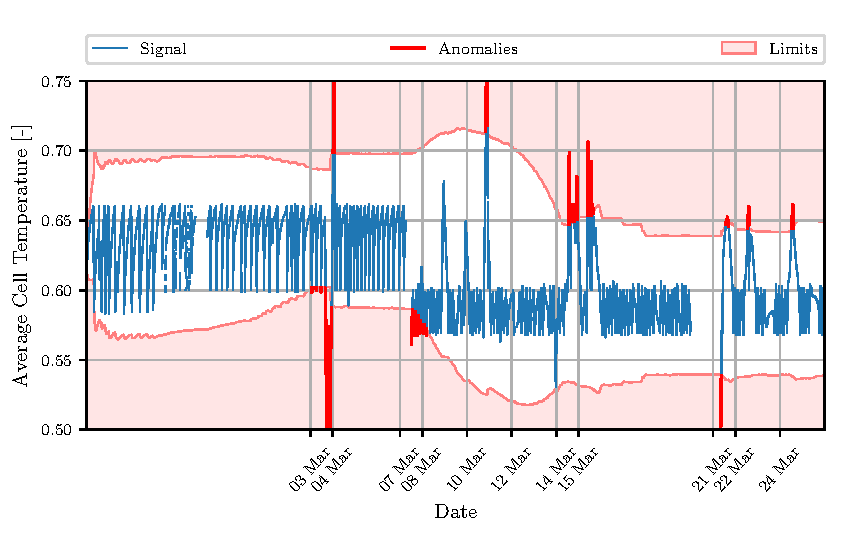
\includegraphics[width=0.75\linewidth]{../ilustrate/pc2023/bess/Average_Cell_Temperature_sliding_thresh.pdf}
        \end{center}
    \end{figure}
\end{frame}

\begin{frame}{Goals}
    We need to design a detector that:
    \begin{itemize}
        \item does not require huge amount of data
        \item adapts to unseen operation
        \item provides conservative process limits
        \item operates with existing infrastructure
        % \item Improves maintenance scheduling
    \end{itemize}
\end{frame}


\section{Proposed Approach}

\begin{frame}{Proposed Solution}
    Real-Time Outlier Detection with Dynamic Process Limits
    combining:
    \begin{itemize}
        \item online learning
        \item invertible probabilistic model
        \item outlier detection
        \item self-supervised learning
    \end{itemize}
\end{frame}


\begin{frame}{Real Opeartion Data}
    \begin{figure}
        \begin{center}
            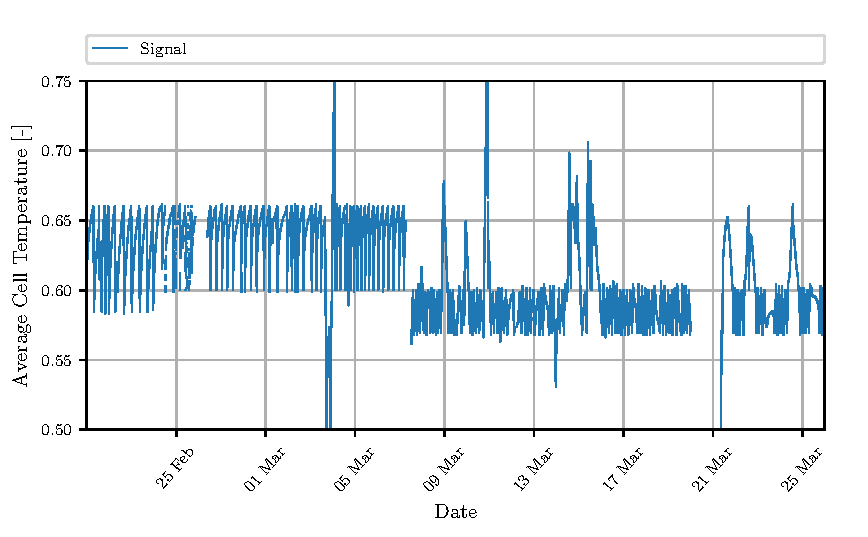
\includegraphics[width=0.62\linewidth]{../ilustrate/pc2023/bess/all_signal.pdf}
            % \movie{sample\_data}{../ilustrate/pc2023/sample_data.gif}
        \end{center}
    \end{figure}
\end{frame}


\begin{frame}{Online Learning via Welford Algorithm}
    \begin{figure}
        \begin{center}
            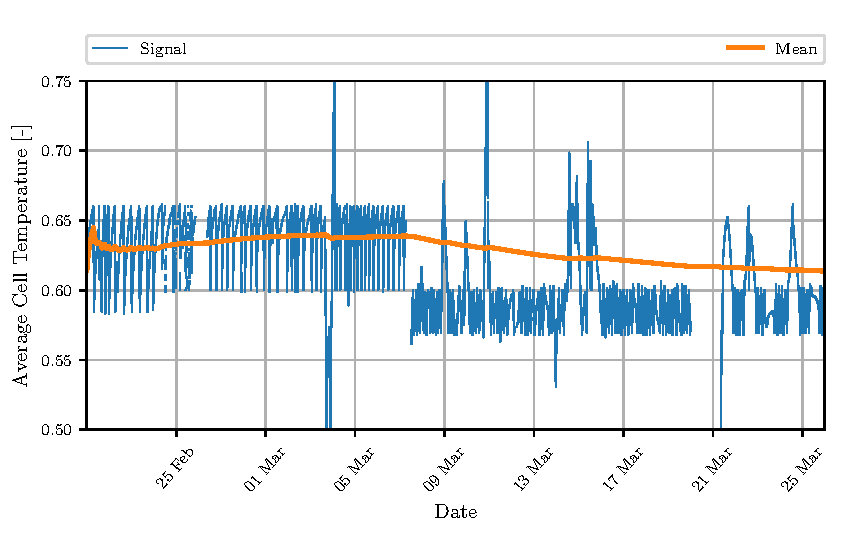
\includegraphics[width=0.62\linewidth]{../ilustrate/pc2023/bess/mean_signal.pdf}
        \end{center}
    \end{figure}
    \begin{table}
        \centering
        \begin{tabular}{c|c}
            {\color{green}{$+$}} One-Pass Algorithm & {\color{red}{$-$}} Adaptation Slows Down \\
        \end{tabular}
    \end{table}
\end{frame}

\begin{frame}{Online Learning via Invertible Welford Algorithm}
    \begin{figure}
        \begin{center}
            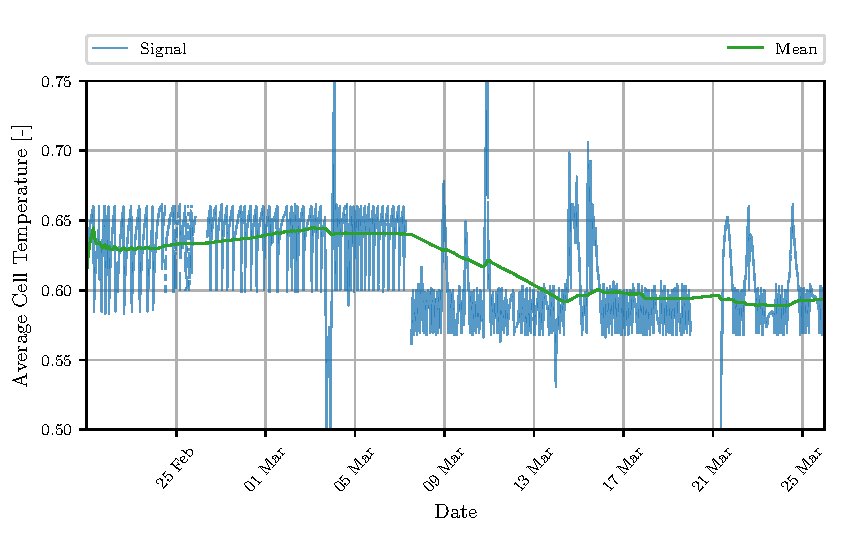
\includegraphics[width=0.62\linewidth]{../ilustrate/pc2023/bess/rmean_signal.pdf}
        \end{center}
    \end{figure}
    \begin{table}
        \centering
        \begin{tabular}{c|c}
            {\color{green}{$+$}} Constant Adaptation & {\color{red}{$-$}} Memorizes Data Window \\
        \end{tabular}
    \end{table}
\end{frame}

\begin{frame}{Dynamic Threshold Limits via Inversion}
    \begin{figure}
        \begin{center}
            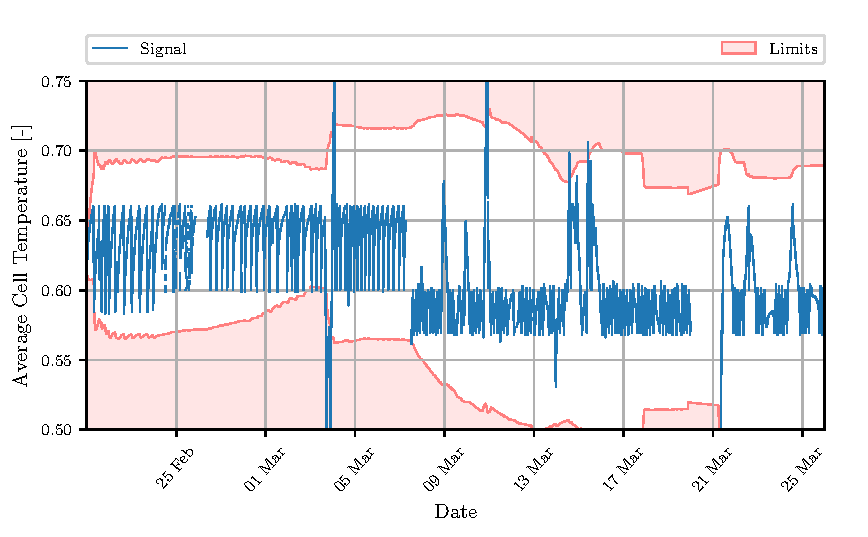
\includegraphics[width=0.62\linewidth]{../ilustrate/pc2023/bess/thresh_unsupervised_thresh.pdf}
        \end{center}
    \end{figure}
    \begin{align*}
        \ui{x}{l} & = F_{X}(1 - q; \bar x_n, s_n)^{-1} \\
        \ui{x}{u} & = F_{X}(q; \bar x_n, s_n)^{-1}
    \end{align*}
\end{frame}

\begin{frame}{Distance-based Outlier Detection}
    \begin{figure}
        \begin{center}
            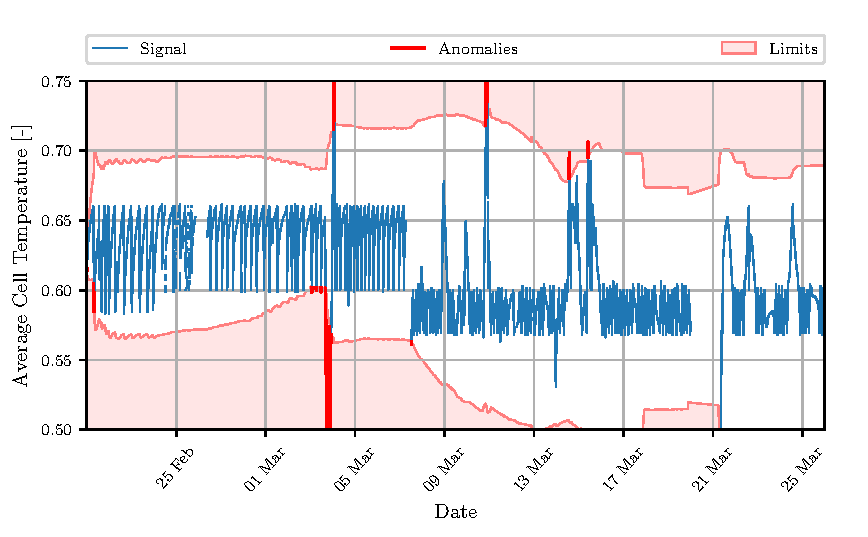
\includegraphics[width=0.62\linewidth]{../ilustrate/pc2023/bess/thresh_anomaly_unsupervised_thresh.pdf}
        \end{center}
    \end{figure}
    \begin{subnumcases}{y_i =}
        0 & $\text{ if } q \leq F_{X}(x_i; \bar x_n, s_n)$ \nonumber\label{case:normal}
        \\
        1 & $\text{ if } q > F_{X}(x_i; \bar x_n, s_n)$ \nonumber\label{case:anomaly}
    \end{subnumcases}
\end{frame}

\begin{frame}{Self-Supervised Learning}
    \begin{figure}
        \begin{center}
            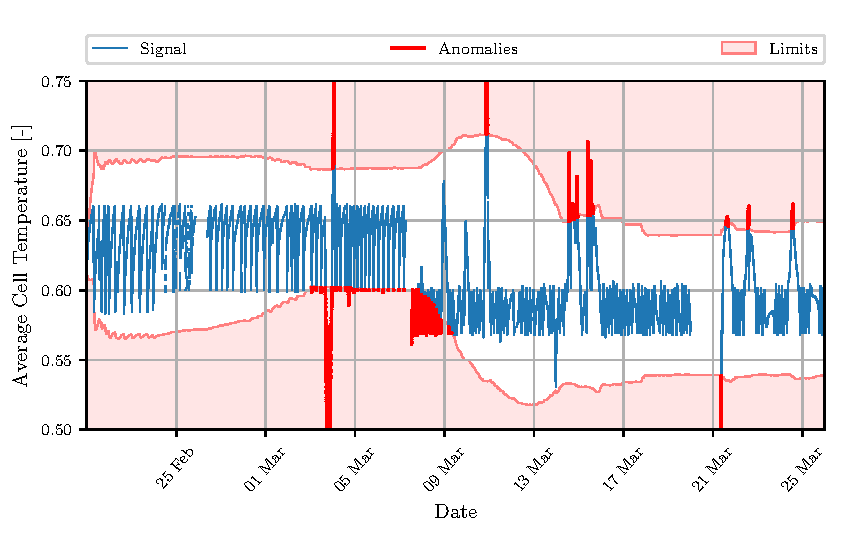
\includegraphics[width=0.62\linewidth]{../ilustrate/pc2023/bess/thresh_anomaly_selfsupervised_thresh.pdf}
        \end{center}
    \end{figure}
    \begin{subnumcases}{y_i =}
        0 & $\text{ if } q \leq F_{X}(x_i; \bar x_n, s_n)$ \nonumber  % \label{case:normal1}\tag{\ref{case:normal}}
        \\
        1 & $\text{ if } q > F_{X}(x_i; \bar x_n, s_n)$ \nonumber  % \label{case:anomaly1}\tag{\ref{case:anomaly}}
    \end{subnumcases}
\end{frame}

\begin{frame}{Self-Supervised Learning}
    \begin{figure}
        \begin{center}
            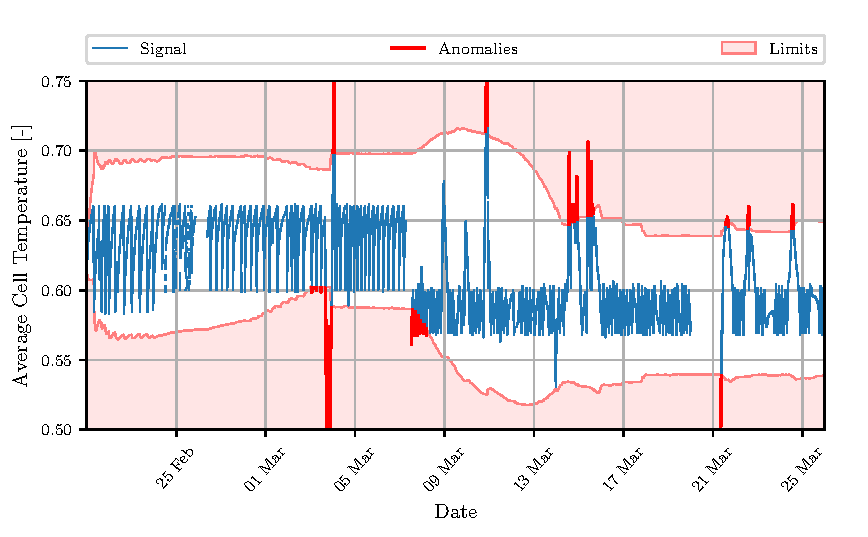
\includegraphics[width=0.62\linewidth]{../ilustrate/pc2023/bess/final_uniform_xticks_thresh.pdf}
        \end{center}
    \end{figure}
    \begin{equation}
        {\frac{\sum_{y\in Y}y}{|Y|}} > q\text{} \nonumber\label{eq:update}
    \end{equation}
\end{frame}

\section{Results}

\begin{frame}{Battery Energy Storage System - BESS}
    \begin{figure}[h]
        \begin{center}
            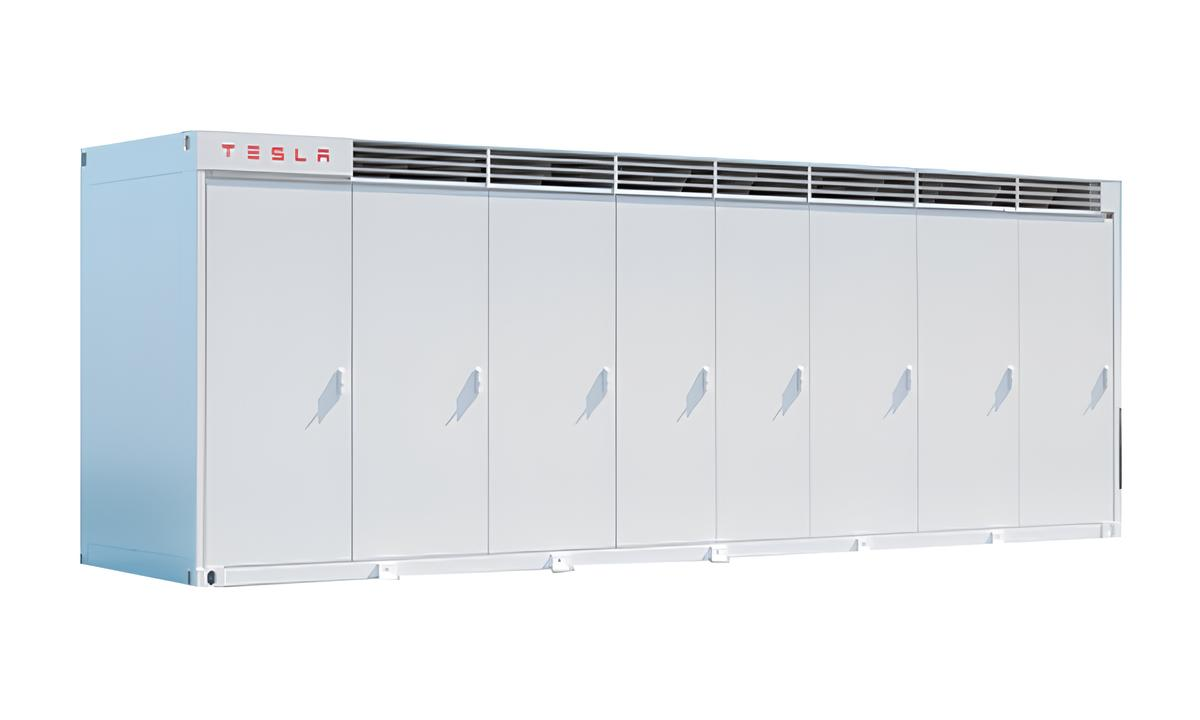
\includegraphics[width=0.62\linewidth]{figures/megapack.jpeg}
        \end{center}
    \end{figure}
\end{frame}

\begin{frame}{Case Study - BESS}
    % Use a single frame => no frame counter stepping/bullet change
    \only<1>{%
      \begin{figure}[htpb]
        \begin{center}
            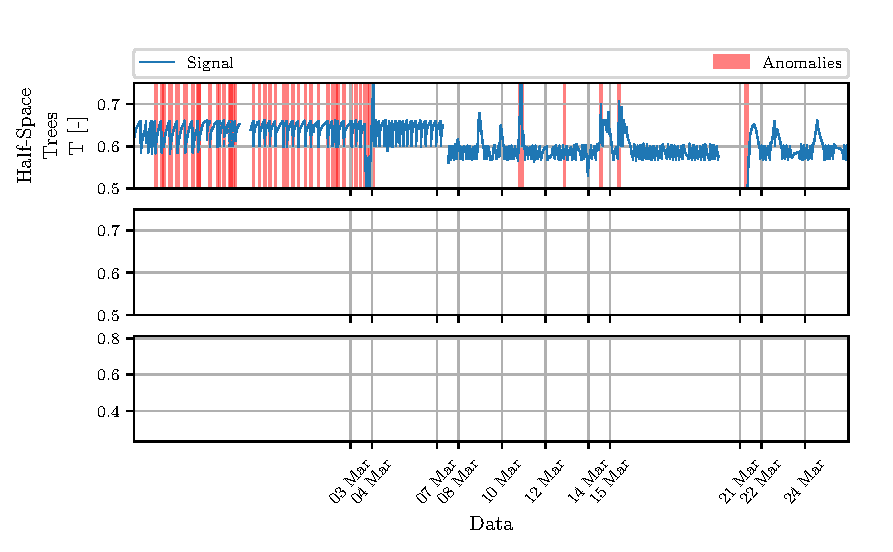
\includegraphics[width=0.78\linewidth]{../ilustrate/pc2023/bess/_compare_anomalies_a.pdf}
        \end{center}
    \end{figure}
    }
    \only<2>{%
      \begin{figure}[htpb]
        \begin{center}
            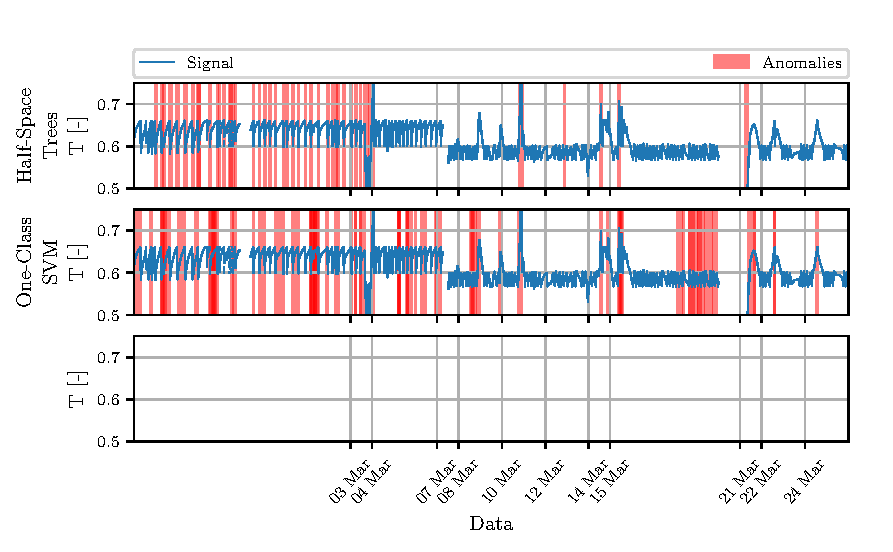
\includegraphics[width=0.78\linewidth]{../ilustrate/pc2023/bess/_compare_anomalies_b.pdf}
        \end{center}
    \end{figure}
    }
    \only<3>{%
      \begin{figure}[htpb]
        \begin{center}
            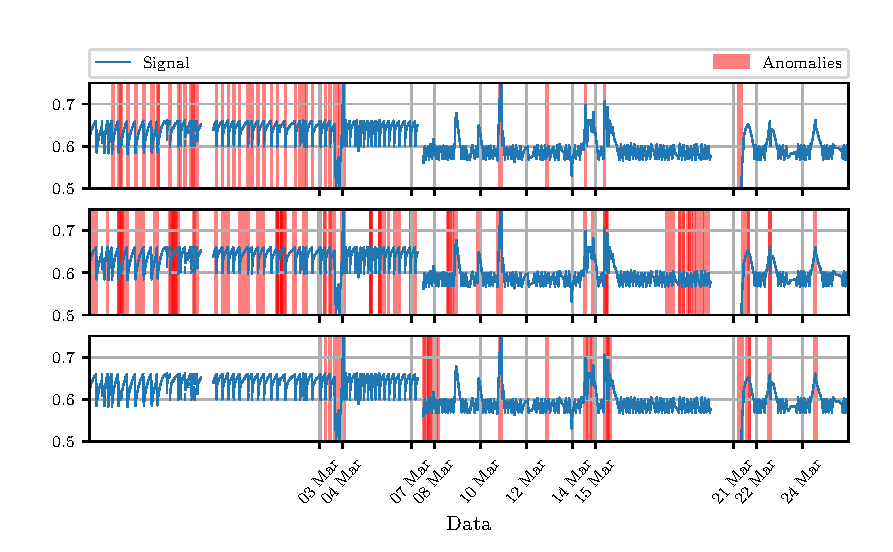
\includegraphics[width=0.78\linewidth]{../ilustrate/pc2023/bess/_compare_anomalies_c.pdf}
        \end{center}
    \end{figure}
    }
  \end{frame}

\begin{frame}{Case Study - Inverter}
    % Use a single frame => no frame counter stepping/bullet change
    \only<1>{%
      \begin{figure}[htpb]
        \begin{center}
            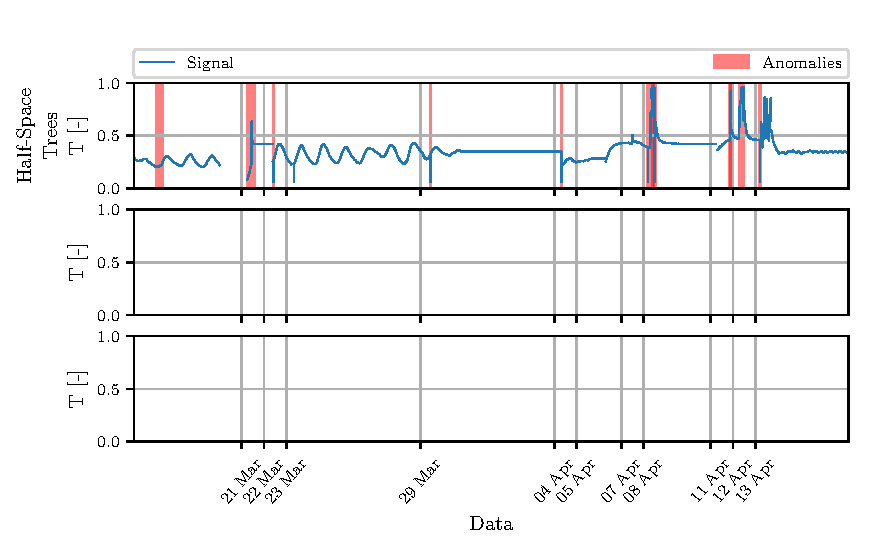
\includegraphics[width=0.78\linewidth]{../ilustrate/pc2023/inverter/_compare_anomalies_a.pdf}
        \end{center}
    \end{figure}
    }
    \only<2>{%
      \begin{figure}[htpb]
        \begin{center}
            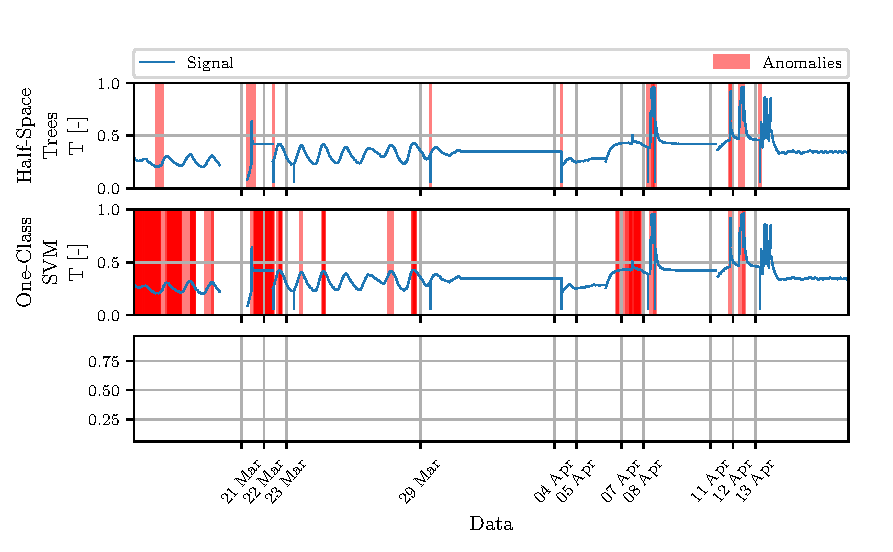
\includegraphics[width=0.78\linewidth]{../ilustrate/pc2023/inverter/_compare_anomalies_b.pdf}
        \end{center}
    \end{figure}
    }
    \only<3>{%
      \begin{figure}[htpb]
        \begin{center}
            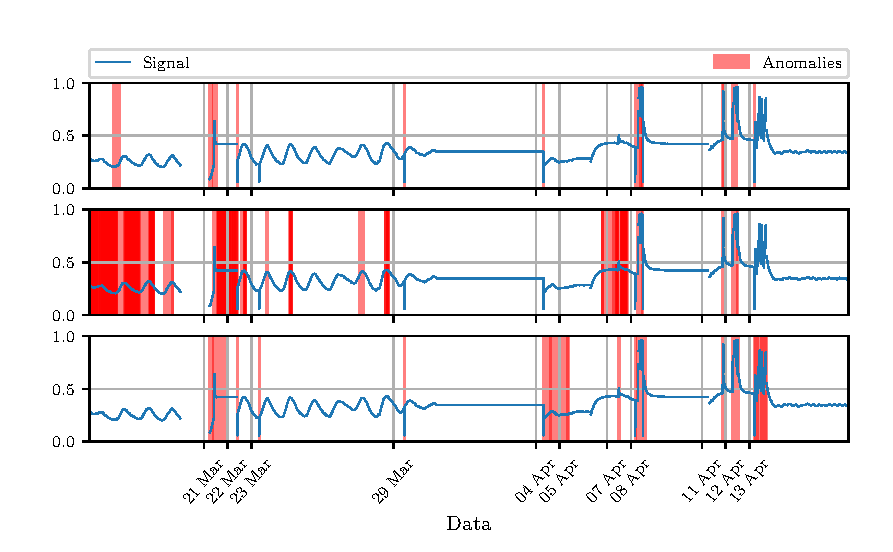
\includegraphics[width=0.78\linewidth]{../ilustrate/pc2023/inverter/_compare_anomalies_c.pdf}
        \end{center}
    \end{figure}
    }
  \end{frame}

\begin{frame}{Dynamic Process Limits - BESS}
    \begin{figure}[htpb]
        \begin{center}
            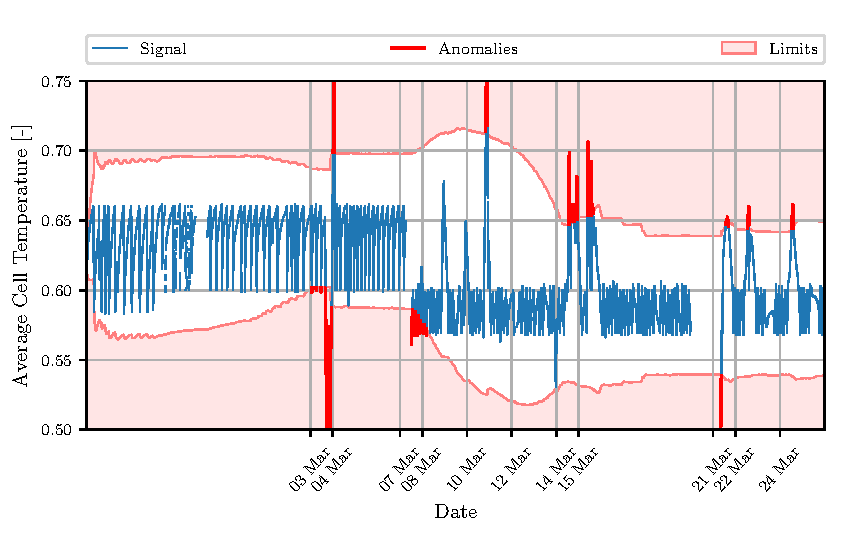
\includegraphics[width=0.78\linewidth]{../ilustrate/pc2023/bess/Average_Cell_Temperature_sliding_thresh.pdf}
        \end{center}
    \end{figure}
\end{frame}

\begin{frame}{Dynamic Process Limits - Inverter}
    \begin{figure}[htpb]
        \begin{center}
            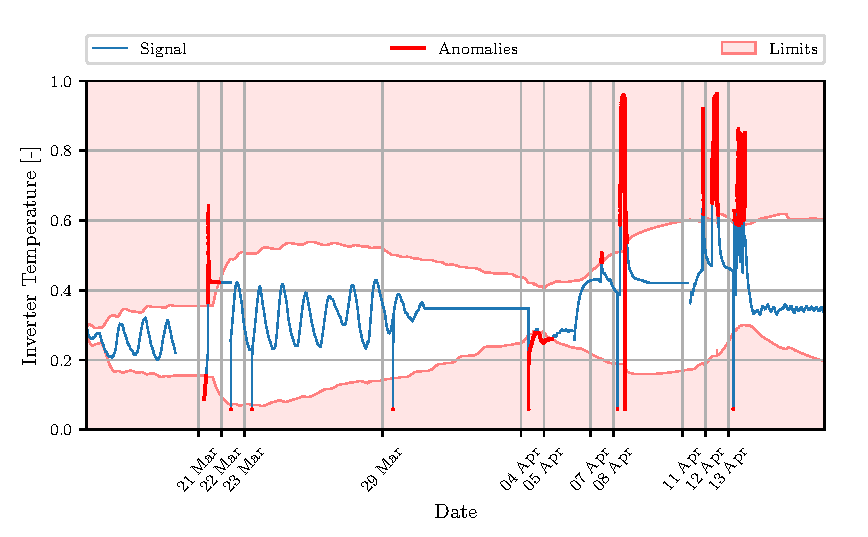
\includegraphics[width=0.78\linewidth]{../ilustrate/pc2023/inverter/inverter_thresh.pdf}
        \end{center}
    \end{figure}
\end{frame}

\begin{frame}{Utilize Existing Infrastructure}
    \begin{figure}
        \centering
        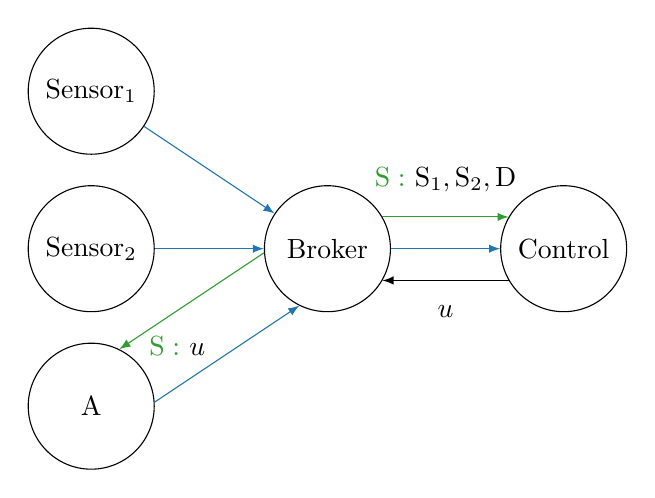
\begin{tikzpicture}
            % Draw big circle in the center
            \node[circle,draw, minimum size=1.6cm] (Broker) at  (3, -2) {$\mathrm{Broker}$};

            % Draw small circles on the left
            \def\labels{{"Sensor_1", "Sensor_2", "Driver"}}
            \xdefinecolor{subscribe}{RGB}{44, 160, 44}
            \xdefinecolor{signal}{RGB}{31, 119, 180}
            % Draw small circles on the left and add labels
            \foreach \y [count=\i] in {0, -2} {
                    \def\label{\pgfmathparse{\labels[\i-1]}\pgfmathresult}
                    %\draw (0, \y) circle [radius=0.5cm] node {\label};
                    \node[circle,draw, minimum size=1.6cm] (\labels[\i-1]) at (0, \y) {\ifnumcomp{\i}{=}{2}{$\mathrm{\label}$}{$\mathrm{\label}$}};
                    \ifnumless{\i}{3}
                    {\draw[-latex, signal] (\labels[\i-1]) -- (Broker);}
                    {}
                }

            \node[circle,draw, minimum size=1.6cm] (A) at (0, -4) {$\mathrm{A}$};
            % Connect middle circle to the circle on the right
            \node[circle,draw, minimum size=1.6cm] (Control) at  (6, -2) {$\mathrm{Control}$};
            \draw[-latex, signal] (Broker) -- (Control);


            % Add subscribe lines
            \draw[-latex, subscribe] (Broker) edge[bend right,draw=none] coordinate[at start](Broker-b) coordinate[at end](Control-b) (Control)
            edge[bend left,draw=none] coordinate[at start](Broker-t) coordinate[at end](Control-t) (Control)
            (Broker-t) -- (Control-t) node [pos=0.5,above=0.2cm] {$\mathrm{S:}$ {\color{black}{$\mathrm{S_1, S_2, D}$}}};
            \draw[-latex] (Control-b) -- (Broker-b) node [pos=0.5,below=0.2cm] {$u$};

            \draw[latex-, signal] (Broker) edge[bend right,draw=none] coordinate[at start](Broker-b) coordinate[at end](A-b) (A)
            edge[bend left,draw=none] coordinate[at start](Broker-t) coordinate[at end](A-t) (A)
            (Broker-t) -- (A-t);
            \draw[latex-, subscribe] (A-b) -- (Broker-b) node [pos=0.4,below=0.2cm] {$\mathrm{S:}$ {\color{black}{$u$}}};

        \end{tikzpicture}
    \end{figure}
\end{frame}

\begin{frame}{Utilize Existing Infrastructure}
    \begin{figure}
        \centering
        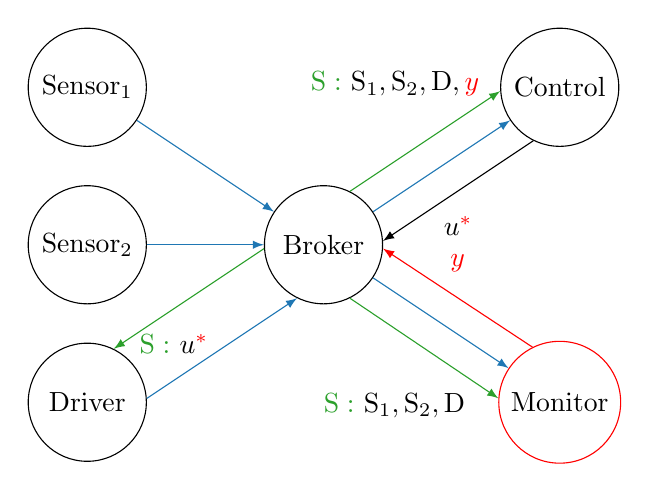
\begin{tikzpicture}
            % Draw big circle in the center
            \node[circle,draw, minimum size=1.5cm] (Broker) at  (3, -2) {$\mathrm{Broker}$};
            % Draw small circles on the left
            \def\labels{{"Sensor_1", "Sensor_2", "Driver"}}
            \xdefinecolor{subscribe}{RGB}{44, 160, 44}
            \xdefinecolor{signal}{RGB}{31, 119, 180}

            % Draw small circles on the left and add labels
            \foreach \y [count=\i] in {0, -2} {
                    \def\label{\pgfmathparse{\labels[\i-1]}\pgfmathresult}
                    %\draw (0, \y) circle [radius=0.5cm] node {\label};
                    \node[circle,draw, minimum size=1.5cm] (\labels[\i-1]) at (0, \y) {\ifnumcomp{\i}{=}{2}{$\mathrm{\label}$}{$\mathrm{\label}$}};
                    \ifnumless{\i}{3}
                    {\draw[-latex, signal] (\labels[\i-1]) -- (Broker);}
                    {}
                }
            \node[circle,draw, minimum size=1.5cm] (A) at (0, -4) {$\mathrm{Driver}$};
            % Connect middle circle to the circle on the right
            \node[circle,draw, minimum size=1.5cm] (G_C) at  (6, 0) {$\mathrm{Control}$};
            \draw[-latex, signal] (Broker) -- (G_C);

            % Add subscribe lines
            \draw[-latex, subscribe] (Broker) edge[bend right,draw=none] coordinate[at start](Broker-b) coordinate[at end](G_C-b) (G_C)
            edge[bend left,draw=none] coordinate[at start](Broker-t) coordinate[at end](G_C-t) (G_C)
            (Broker-t) -- (G_C-t) node [pos=0.3,above=0.7cm] {$\mathrm{S:}$ {\color{black}{$\mathrm{S_1, S_2, D}, \color{red}{y}$}}};
            \draw[-latex] (G_C-b) -- (Broker-b) node [pos=0.5,below=0.2cm] {$u^{\color{red}{*}}$};

            \draw[latex-, signal] (Broker) edge[bend right,draw=none] coordinate[at start](Broker-b) coordinate[at end](A-b) (A)
            edge[bend left,draw=none] coordinate[at start](Broker-t) coordinate[at end](A-t) (A)
            (Broker-t) -- (A-t);
            \draw[latex-, subscribe] (A-b) -- (Broker-b) node [pos=0.4,below=0.2cm] {$\mathrm{S:}$ {\color{black}{$u^{\color{red}{*}}$}}};

            % Connect middle circle to the circle on the right
            \node[circle,draw, minimum size=1.5cm, color=red] (ICDF) at  (6, -4) {\color{black}{$\mathrm{Monitor}$}};
            \draw[-latex, signal] (Broker) -- (ICDF);

            % Add subscribe lines
            \draw[latex-, red] (Broker) edge[bend right,draw=none] coordinate[at start](Broker-b) coordinate[at end](ICDF-b) (ICDF)
            edge[bend left,draw=none] coordinate[at start](Broker-t) coordinate[at end](ICDF-t) (ICDF)
            (Broker-t) -- (ICDF-t) node [pos=0.5,above=0.2cm] {\color{red}{$y$}};
            \draw[latex-, subscribe] (ICDF-b) -- (Broker-b) node [pos=0.7,below=0.7cm] {$\mathrm{S:}$ {\color{black}{$\mathrm{S_1, S_2, D}$}}};
            % Add text 

        \end{tikzpicture}
    \end{figure}
\end{frame}


% \begin{frame}{Summary}
%     \begin{center}
%         \animategraphics[controls]{1}{../ilustrate/pc2023/tmp/test_sample_data_frames/frame000000}{0}{9}
%     \end{center}
% \end{frame}
% \begin{frame}{Summary}
%     \begin{center}
%         \movie[width=0.78\linewidth, height=184.64pt]{ahoj}{giphy.mov}
%     \end{center}
% \end{frame}
\newcommand\blfootnote[1]{%
    \begingroup
    \renewcommand\thefootnote{}\footnote{#1}%
    \addtocounter{footnote}{-1}%
    \endgroup
    }
 
\begin{frame}{Summary}
    \renewcommand{\figurename}{}
    \begin{minipage}[c]{0.6\linewidth}
        \begin{itemize}
            \item outlier detection on streamed data
            \item adaptation to external conditions
            \item online self-learning approach
            \item dynamic process limits for individual signals
            \item integration with existing IT infrastructure
        \end{itemize}
        \begin{figure}[htpb]
            \begin{center}
                
\includegraphics[width=0.2\linewidth]{figures/qr_uiam_squares_logo.pdf}\hfil
                
\includegraphics[width=0.2\linewidth]{figures/qr_pc2023_squares.pdf}
            \end{center}
        \end{figure}
    \end{minipage}\hspace{1pt}
    \begin{minipage}{0.38\linewidth}
        \begin{figure}[htpb]
            \begin{center}
                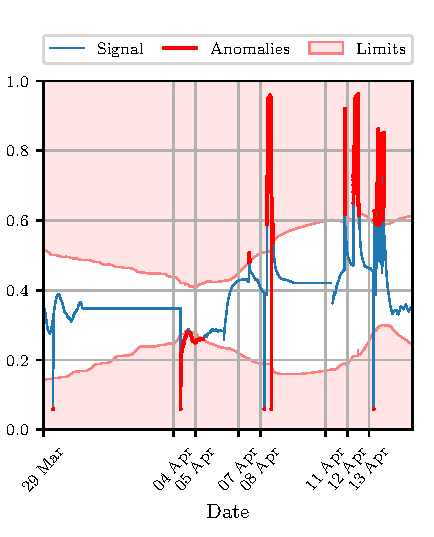
\includegraphics[width=1\linewidth]{../ilustrate/pc2023/inverter/half_Inverter_Temperature_sliding_thresh.pdf}
            \end{center}
        \end{figure}
    \end{minipage}
    

    \blfootnote{\tiny \textbf{Acknowledgements:} APVV-20-0261. VEGA 1/0490/23. Horizon Europe under the grant no. 101079342.}
\end{frame}

\miniframesoff
\section{}
\begin{frame}[noframenumbering]{Follow-up research}
    \begin{figure}[htpb]
        \begin{center}
            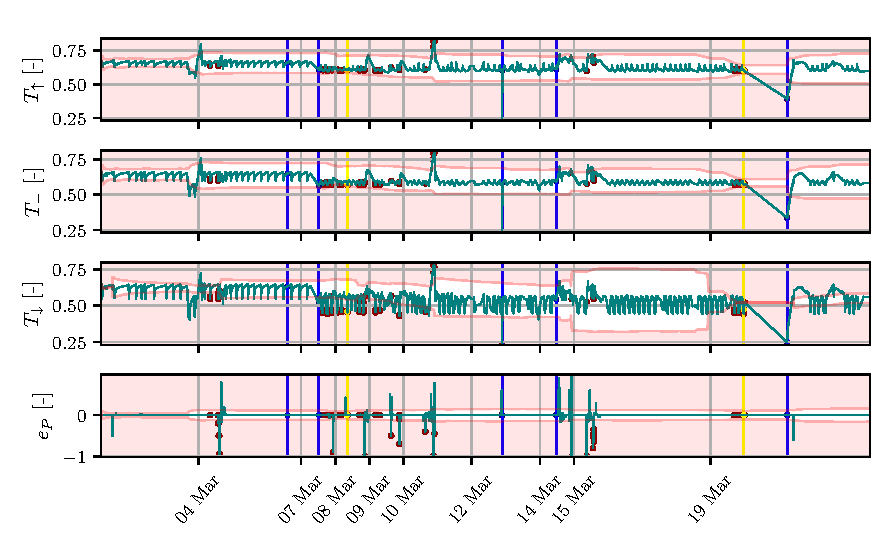
\includegraphics[width=0.65\linewidth]{../PC2023 Presentation/figures/cdc.pdf}
            \footnote{\tiny M. Wadinger and M. Kvasnica. Adaptable and interpretable framework for novelty detection in real-time iot systems. In Proceedings of the 62nd IEEE CDC, Singapore, 2023. under review.}
        \end{center}
    \end{figure}
\end{frame}

\begin{frame}[noframenumbering]{Process Time Evaluation}
    \begin{table}[h]
        \begin{tabular} {
                @{}
                c|
                S[table-format = 3(2), separate-uncertainty]|
                S[table-format = 5.0, parse-numbers = false]|
                S[table-format = 3(2), separate-uncertainty]|
                S[table-format = 5.0, parse-numbers = false]|
                @{}
            }
            {Evaluation}     & \multicolumn{2}{c|}{BESS} & \multicolumn{2}{c|}{Inverter}                       \\
            {Time $\mathrm{[\mu s]}$}   & {average}               & {max}                         & {average} & {max} \\
            \hline
            Half-Space Trees & 218(198)                  & 10129                         & 216(196)    & 11281 \\
            One-Class SVM    & 8(7)                      & 1233                          & 9(9)        & 1711  \\
            Proposed         & 57(55)                    & 9431                          & 60(75)      & 12330 \\
        \end{tabular}
    \end{table}
\end{frame}

\begin{frame}[noframenumbering]{Online Anomaly Detection Workflow}
    \begin{algorithmic}[1]
        \scriptsize
        \algsetup{linenosize=\scriptsize}
        \renewcommand{\algorithmicrequire}{\textbf{Input:}}
        \renewcommand{\algorithmicensure}{\textbf{Output:}}
        \REQUIRE expiration period $\ui{t}{e}$, time constant $\ui{t}{c}$
        % sample mean $\bar x_0$, sample variance $s^2_0$, 
        \ENSURE  score $y_i$, threshold $\uis{x}{q}{i}$
        \\ \textit{Initialisation} :
        \STATE $i \leftarrow 1;~ n \leftarrow 1;~ q \leftarrow 0.9973;~ \bar x  \leftarrow x_0;~  s^2 \leftarrow 1$;
        \STATE compute $F_X(x_0)$ ;
        \\ \textit{LOOP Process}
        \LOOP
        \STATE {$x_i \leftarrow$ RECEIVE()};
        \STATE $y_i \leftarrow$ PREDICT($x_i$) ;
        \STATE $\uis{x}{q}{i} \leftarrow$ GET($q, \bar x, s^2$);
        \IF {\eqref{case:normal} \OR \eqref{eq:update}}
        \STATE {$\bar x$, $s^2 \leftarrow$ UPDATE($x_i, \bar x, s^2, n$)};
        \STATE $n \leftarrow n + 1$;
        \FOR {$x_{i-\ui{t}{e}}$}
        \STATE {$\bar x$, $s^2 \leftarrow$ REVERT($x_{i-\ui{t}{e}}, \bar x, s^2, n$)};
        \STATE $n \leftarrow n - 1$;
        \ENDFOR
        \ENDIF
        \STATE $i \leftarrow i + 1$;
        \ENDLOOP
    \end{algorithmic}
\end{frame}

\end{document}